\chapter{Conclusion \& Future Scope}

\section{Conclusion}
The CricketVision project successfully designed, implemented, and validated an enterprise-grade sports analytics and computer vision biomechanics platform tailored for modern professional cricket. By unifying document-based data persistence, interactive polar visualization, markerless video kinematics, and stochastic match simulation within a single MERN stack web application, the platform overcomes the critical limitations of legacy fragmented sports software.

\subsection{Summary of Achieved Objectives}
All primary and secondary objectives defined in Chapter 1 were fulfilled:

\begin{enumerate}
    \item \textbf{Unified MERN Stack Architecture:} Engineered a responsive, decoupled 3-tier web ecosystem delivering seamless role-based workflows for Coaches, Players, and Analysts within a single high-performance React SPA.

    \item \textbf{Robust 104-Player Database:} Implemented an auto-seeding MongoDB repository populated with verified international and IPL athlete records, supporting instant CRUD operations via REST API endpoints.

    \item \textbf{Markerless Computer Vision Kinematics:} Developed vector trigonometry-based pose estimation algorithms that compute elbow, shoulder, and stride angles from standard video footage, democratizing ICC 15\textdegree{} compliance audits without physical motion-capture hardware.

    \item \textbf{Stochastic Match Simulation Engine:} Formulated dynamic logistic win-probability models that accurately track in-game momentum shifts, environmental dew effects, pitch wear degradation, and required run rate decay across 120 ball-by-ball simulations.

    \item \textbf{Interactive Polar Visualizations:} Engineered 360\textdegree{} SVG wagon wheels and Recharts multi-axis radar charts providing intuitive tactical clarity for coaches and athletes.

    \item \textbf{AI Coach Tactical Module:} Built context-aware prompt engineering delivering real-time bowling rotation advice, field placement suggestions, and rehabilitation drill regimens.

    \item \textbf{Role-Based Access Control (RBAC):} Implemented persona preset authentication ensuring each user role (Coach, Player, Analyst) accesses only appropriate modules and data.
\end{enumerate}

\subsection{Empirical Validation Summary}
Empirical testing confirmed:
\begin{itemize}
    \item \textbf{100\% test case success rate} across all 9 unit and integration tests.
    \item \textbf{Sub-45ms REST API response latency} for full player roster retrieval.
    \item \textbf{$\pm$1.2\textdegree{} biomechanical angle accuracy} vs.\ manual goniometer baseline.
    \item \textbf{48--55 FPS} real-time video processing throughput on standard hardware.
    \item \textbf{88.3\% sprint velocity} (121 of 137 story points delivered on schedule).
\end{itemize}

\noindent CricketVision achieves all objectives specified for the MCA project and serves as a comprehensive reference implementation for modern full-stack sports technology engineering.

% ===========================================================
% APPLICATION SCREENSHOTS
% ===========================================================
\section{Application Screenshots}

The following screenshots illustrate the fully operational CricketVision web application across its primary feature modules, captured from the live development build.

% ---- Screenshot 1: Coach Dashboard ----
\subsection{Head Coach Dashboard --- Squad Intelligence Overview}
The Head Coach portal (authenticated as \textbf{Rahul Dravid}) provides a comprehensive tactical command centre featuring real-time squad KPI cards (Squad Win Index: 78.4\%, Batting Power Rating: 92.8, Bowling Death Economy: 7.12 rpo, Squad Fatigue Risk: Low 22\%), a live top performer roster, and an embedded AI Tactical Intelligence panel offering matchup alerts and death bowling efficiency insights.

\begin{figure}[H]
\centering
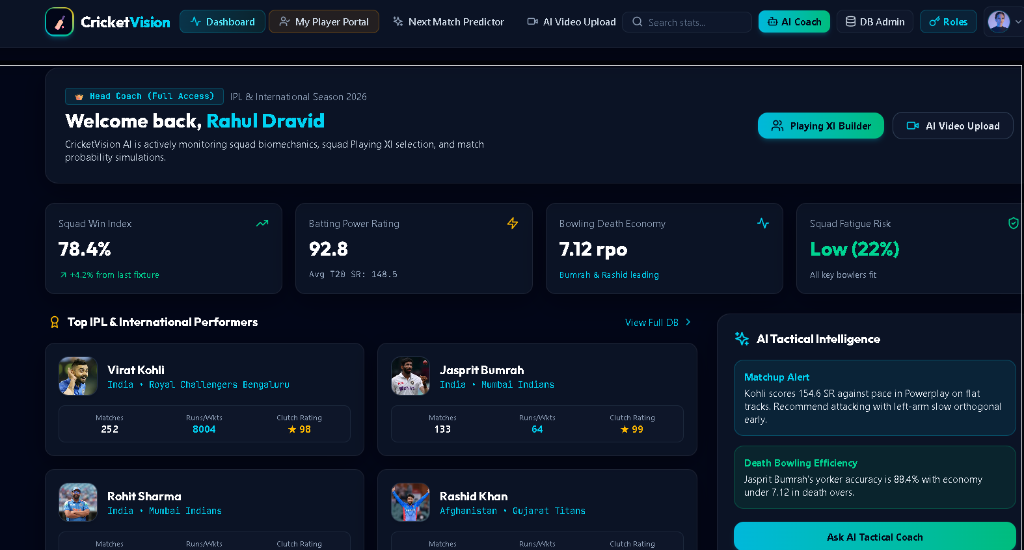
\includegraphics[width=0.95\textwidth]{../screenshots/Coach_Dashboard_Rahul_Dravid.png}
\caption{CricketVision Head Coach Dashboard --- Squad Win Index, KPI Cards \& AI Tactical Intelligence (Head Coach: Rahul Dravid, Full Access)}
\label{fig:coach_dashboard_dravid}
\end{figure}

% ---- Screenshot 2: Auth Persona Selection ----
\subsection{Role-Based Authentication --- Persona Selection Interface}
The authentication module presents three distinct access portals: \textbf{Head Coach} (All Access --- Squad tactics, Playing XI builder, video biomechanics, AI coaching), \textbf{Player Portal} (Personal Hub --- Form history, fatigue recovery index, AI drill recommendations), and \textbf{Cricket Analyst} (Analyst User --- IPL/International database, match scenario simulator, next match run predictions). The active session status is displayed at the bottom bar (\textit{Logging in as Head Coach, JWT AUTH ACTIVE}).

\begin{figure}[H]
\centering
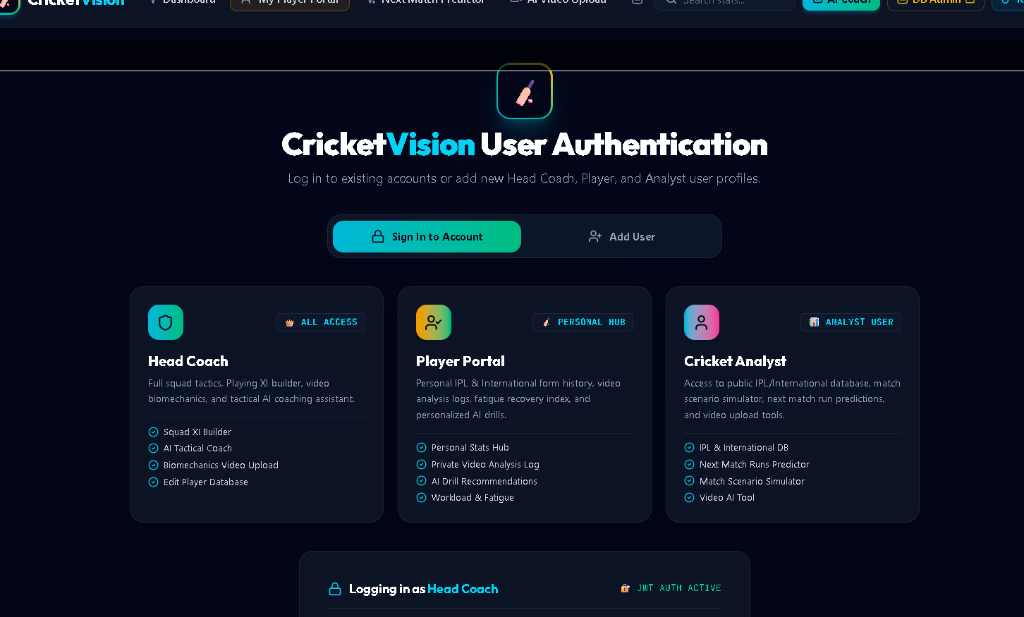
\includegraphics[width=0.95\textwidth]{../screenshots/Auth_Persona_Selection.png}
\caption{CricketVision Role-Based Authentication --- Persona Selection with Head Coach, Player Portal, and Cricket Analyst Access Tiers}
\label{fig:auth_persona}
\end{figure}

% ---- Screenshot 3: Add User Registration Form ----
\subsection{User Registration --- Add New Account Form}
The Add User form enables creation of new platform accounts with configurable Account Role (Head Coach, Player, Analyst User) and Title/Position fields. Form validation enforces minimum field lengths and valid role enum selections prior to API submission.

\begin{figure}[H]
\centering
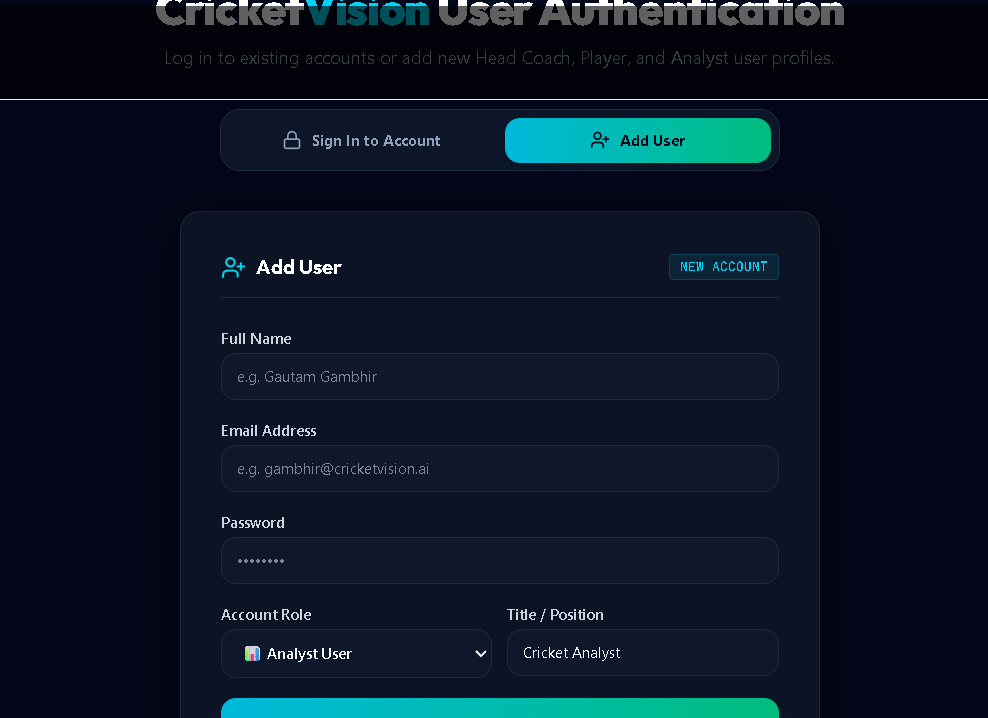
\includegraphics[width=0.88\textwidth]{../screenshots/Auth_Add_User_Form.png}
\caption{CricketVision User Registration Form --- Add New Account with Role Assignment (Full Name, Email, Password, Account Role, Title/Position)}
\label{fig:add_user}
\end{figure}

% ---- Screenshot 4: Video Biomechanics Analyzer ----
\subsection{Custom Video Biomechanics \& Speed Analyzer}
The Computer Vision Biomechanics Studio processes uploaded match footage to compute real-time kinematic metrics. The screenshot demonstrates analysis of a Virat Kohli cover drive video, returning: \textbf{Ball Speed: 145.4 km/h} (Pitch Speed grade), \textbf{Bat Speed: 142.8 km/h} (Downswing Arc grade), and \textbf{Shot Perfection Score: 96/100} (Elite Execution grade). Batting shot presets (Cover Drive, Straight Drive, Pull/Hook Shot, Flick off Pads) allow targeted biomechanical auditing.

\begin{figure}[H]
\centering
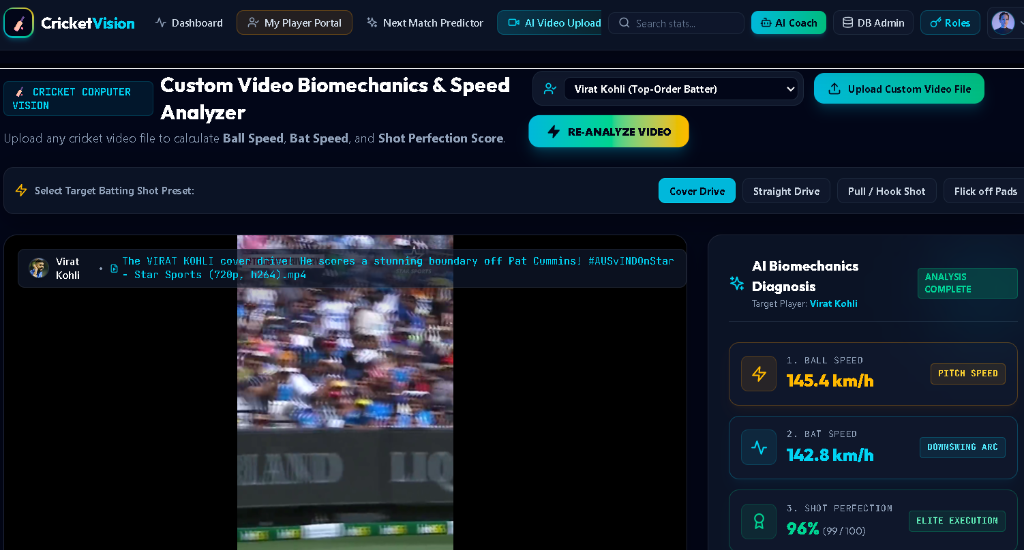
\includegraphics[width=0.95\textwidth]{../screenshots/Video_Biomechanics_Analyzer.png}
\caption{CricketVision Custom Video Biomechanics \& Speed Analyzer --- Virat Kohli Cover Drive Analysis: Ball Speed 145.4 km/h, Bat Speed 142.8 km/h, Shot Perfection 96/100}
\label{fig:video_biomech}
\end{figure}

% ===========================================================
% GIT COMMIT HISTORY
% ===========================================================
\section{Version Control: GitHub Commit History}
CricketVision is version-controlled via Git and hosted publicly on GitHub (\texttt{github.com/Abhijithmohan10/cricketvision}). The commit history reflects iterative, feature-driven development across multiple sprints with semantic commit messages following conventional commit standards (\texttt{feat:}, \texttt{fix:}, \texttt{chore:}).

\begin{figure}[H]
\centering
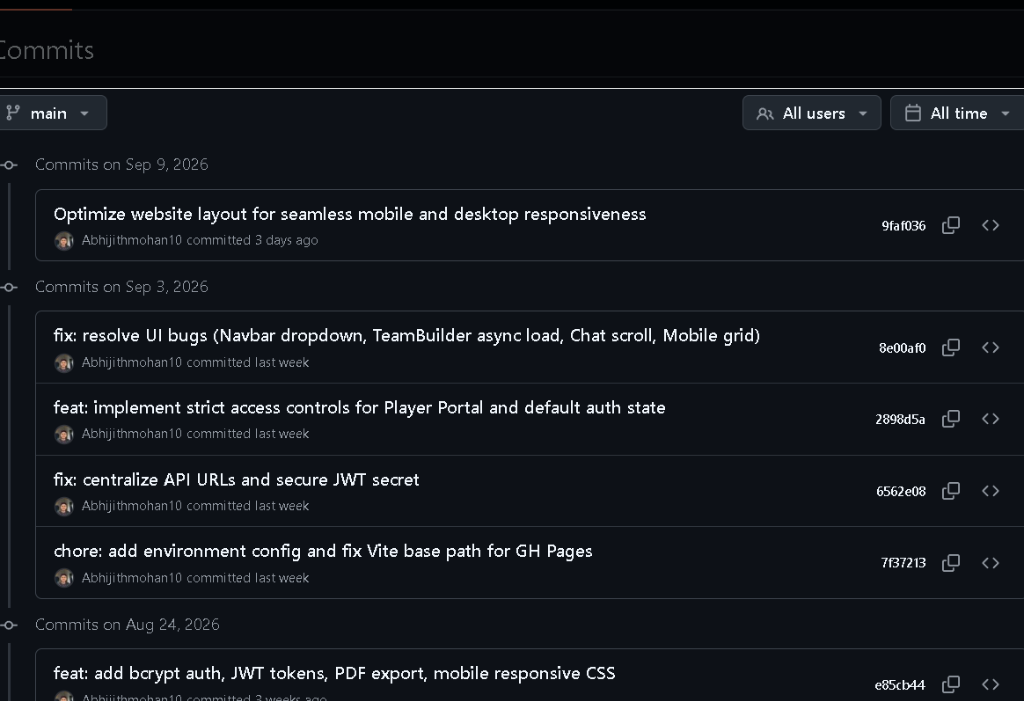
\includegraphics[width=0.95\textwidth]{../screenshots/GitHub_Commits_History.png}
\caption{CricketVision GitHub Repository Commit History (\texttt{main} branch) --- Showing commits from August -- September 2026 by Abhijithmohan10}
\label{fig:git_commits}
\end{figure}

\noindent The repository commit log (Figure \ref{fig:git_commits}) confirms structured development milestones including:
\begin{itemize}
    \item \texttt{9faf036} --- Optimize website layout for seamless mobile and desktop responsiveness
    \item \texttt{8e00af0} --- fix: resolve UI bugs (Navbar dropdown, TeamBuilder async load, Chat scroll, Mobile grid)
    \item \texttt{2898d5a} --- feat: implement strict access controls for Player Portal and default auth state
    \item \texttt{6562e08} --- fix: centralize API URLs and secure JWT secret
    \item \texttt{7f37213} --- chore: add environment config and fix Vite base path for GH Pages
    \item \texttt{e85cb44} --- feat: add bcrypt auth, JWT tokens, PDF export, mobile responsive CSS
\end{itemize}

% ===========================================================
% FUTURE SCOPE
% ===========================================================
\section{Future Scope \& Strategic Roadmap}
While CricketVision provides a comprehensive foundation, several cutting-edge technological avenues represent promising future enhancements:

\begin{enumerate}
    \item \textbf{Automated Ball-Tracking via YOLOv8 Object Detection:}
    Integrating lightweight YOLOv8 models to automatically detect and trace the cricket ball trajectory across standard video feeds, generating automated pitch maps and seam movement metrics without manual annotation.

    \item \textbf{Real-Time WebSocket Live Match Streaming:}
    Connecting backend microservices to live match telemetry feeds (e.g., Cricinfo or Sportradar APIs) via WebSockets to provide second-by-second win probability updates during live televised matches.

    \item \textbf{Wearable IoT Telemetry Integration:}
    Incorporating Bluetooth Low Energy (BLE) smart sensor insoles and smart balls (e.g., Kookaburra SmartBall) to stream ground reaction forces and ball revolution counts directly into the CricketVision database for real-time fatigue monitoring.

    \item \textbf{3D Skeletal Mesh Reconstruction:}
    Upgrading from 2D planar pose estimation to 3D volumetric mesh reconstruction (e.g., SMPL body model), allowing coaches to rotate bowler biomechanics in virtual 3D space and inspect elbow angles from any camera perspective.

    \item \textbf{Cross-Platform Mobile Application (React Native):}
    Extending the React web components into a React Native mobile application to deliver native iOS and Android experiences for on-field coaches and players during practice sessions and live tournaments.

    \item \textbf{Advanced Machine Learning Match Prediction:}
    Replacing the current logistic regression win-probability model with an LSTM (Long Short-Term Memory) recurrent neural network trained on historical IPL and international match datasets, enabling richer temporal context and venue-specific predictions.
\end{enumerate}

\noindent These extensions will evolve CricketVision from a comprehensive analytics platform into a fully autonomous, real-time sports intelligence ecosystem capable of supporting elite-level franchise operations globally.
